\chapter{Background}

\section{High dimensional data issues}
Working with \textit{high dimensional} (HD)\footnote{A small remark on terminology: In this work, I will use the term High Dimensional (HD) data for any dataset with a number of features larger than 256. In other literature, an HD dataset is often defined as a dataset where N (number of data points) is larger than D (number of features - or dimensions). Although I touch on small N datasets, this work mainly does not discuss these specifically.} data presents many issues, often described as "the curse of dimensionality." These range from exponentially increasing the number of samples needed to obtain the same point density, through uniformly distributed points being on average further and further away, to spheres being very "pointy".

Issues caused by HD datasets also have a noticeable impact on machine learning models. These require amounts of data linearly increasing with the factor of 5 [\cite{Koutroumbas}]. Otherwise, the predictive power of a classifier or regressor decreases with higher dimensionality [\cite{McLachlan}, \cite{Trunk}]. This can be apparent, especially in dense neural networks, where the number of parameters will rise with the input dimension, which, in turn, requires more data or additional regularization methods.

\section{Existing approaches for feature selection}
There are two main approaches to dealing with HD datasets. We can transform the given problem into a lower-dimensional setting or use just a projection into a lower-dimensional space (by using only some selected features).

Techniques transforming problems into lower-dimensional spaces are called \textit{Dimensionality Reduction} (DR) techniques. The one most commonly used is principal component analysis (PCA). Still, neural networks have shown the ability to provide DR by themselves, such as variational autoencoders (very well described by \cite{vae}), making using DR techniques before classifiers in some instances redundant.

Another approach for applying machine learning models to high-dimensional data is removing some features based on predefined criteria. There are two general approaches to solving this issue. The first one is \textit{wrapper methods}, which evaluates the whole trained model with some features removed. The second one is \textit{filter methods}, which uses some non-model metric to select the most relevant features. These methods are mainly used for model size and inference-time reduction, as they usually don't bring much performance improvements. As such, these are not evaluated as baselines in this work.

With technological advancements in the past years, these methods have often been omitted, as training a model on the whole feature set has become easier.

\section{Images - high dimensional data}
Humans cannot easily perceive HD data in a vector-like way. Still, we are used to another data format that is much more dense. These are images. Compared to vector-based datasets, images have much more data per sample. For example, a black-and-white image with a resolution of 256 x 256 contains over 65k individual data points. 

State-of-the-art technologies for image classification and other image-related tasks do not use feature selection techniques, at least since AlexNet (\cite{AlexNet}), as they've moved to a solution more integrated into the model's architecture using \textit{Convolutional Neural Networks} \ac{CNN}. These neural networks significantly decrease the needed amount of trained parameters in a model by utilizing common filters commonly applied to the input image's individual parts.

We reuse CNNs to potentially achieve higher performance in our models with data transformed into an image, which also provides us with an easier visualization of a given data point. 

\subsection{Converting vectors to images}
Vectors can be directly converted to images (matrices) by reshaping them to the desired shape. This doesn't significantly improve model performance, as images contain positional relationships, which \ac{CNN}s take full advantage of. To utilize this aspect of the CNN architecture, we also need to transform vectors into images non-trivially. There are multiple proposed algorithms for converting vector data into images. For example, \cite{Zhu2021} propose the IGTD algorithm, which uses an edited distance matrix for the image transformation. DeepInsight proposed by \cite{Sharma2019} firstly finds the location of features based on a DR technique and then creates images by averaging the feature values per pixel. Other approaches have been proposed, such as \cite{omicsmapnet} or \cite{Shneiderman1992}. In this work, I explore a method for rearranging features into images proposed in \cite{REFINED} and compare it to other state-of-the-art approaches.

There was one main criterion when choosing a dataset for this task. It needed enough features ($> 256$) for images transformed by REFINED to make sense. Based on this requirement, an excellent data source has presented itself as data created by P2Rank - a software offered by \cite{P2RANK}. In this chapter, I'll first explain in detail the origin of the data, including the chemical background, the importance of the problem in the real world, and the precise way the data was created. Then, I'll explain this dataset from a data science or machine learning point of view, with all relevant information included. 

\section{Ligand Binding site prediction}

One dataset presented itself that fits all of these criteria. I needed enough features ($> 256$) for vectors to be transformable into images (images of size 3x3 do not make sense). Based on this requirement, looking at the Ligand Binding Site (LBS) prediction on proteins made complete sense. Now, let's look at what this problem tries to solve and understand the main concepts of the dataset I used in the experiments. 

\subsection{Protein structure}
\label{Protein_description}

Proteins are organic macromolecules. They are long chains of smaller molecules called amino acids, with up to hundreds in a chain.

An amino acid is a small molecule containing an amino group (N-terminus) and a carboxyl group (C-terminus). In a protein, individual amino acids are connected by a peptide bond that connects these two groups of adjacent amino acids.

The instructions for making a protein are stored in DNA. Transcribing the genetic code produces mRNA, which serves as a template for the protein. Ribosome units are mounted on this template, and with their help, the individual amino acids forming the protein are connected. As the protein exits the ribosome, folding occurs to ensure the correct 3D structure of the protein. Larger proteins do not fold independently but need auxiliary proteins, so-called chaperones, to fold correctly. The resulting structure is essential for the protein's biological activity and can be used to predict the ligandability of a substance.

There are four ways to view the arrangement of the protein, called structures. They all represent the same protein but consider it from a different point of view.

The primary structure represents the order of amino acids in the sequence, which is determined by the peptide bonds in the sequence. In this structure, each protein is described by its string of amino acids as can be seen in ~\ref{fig:primary}

\begin{figure}
    \centering
    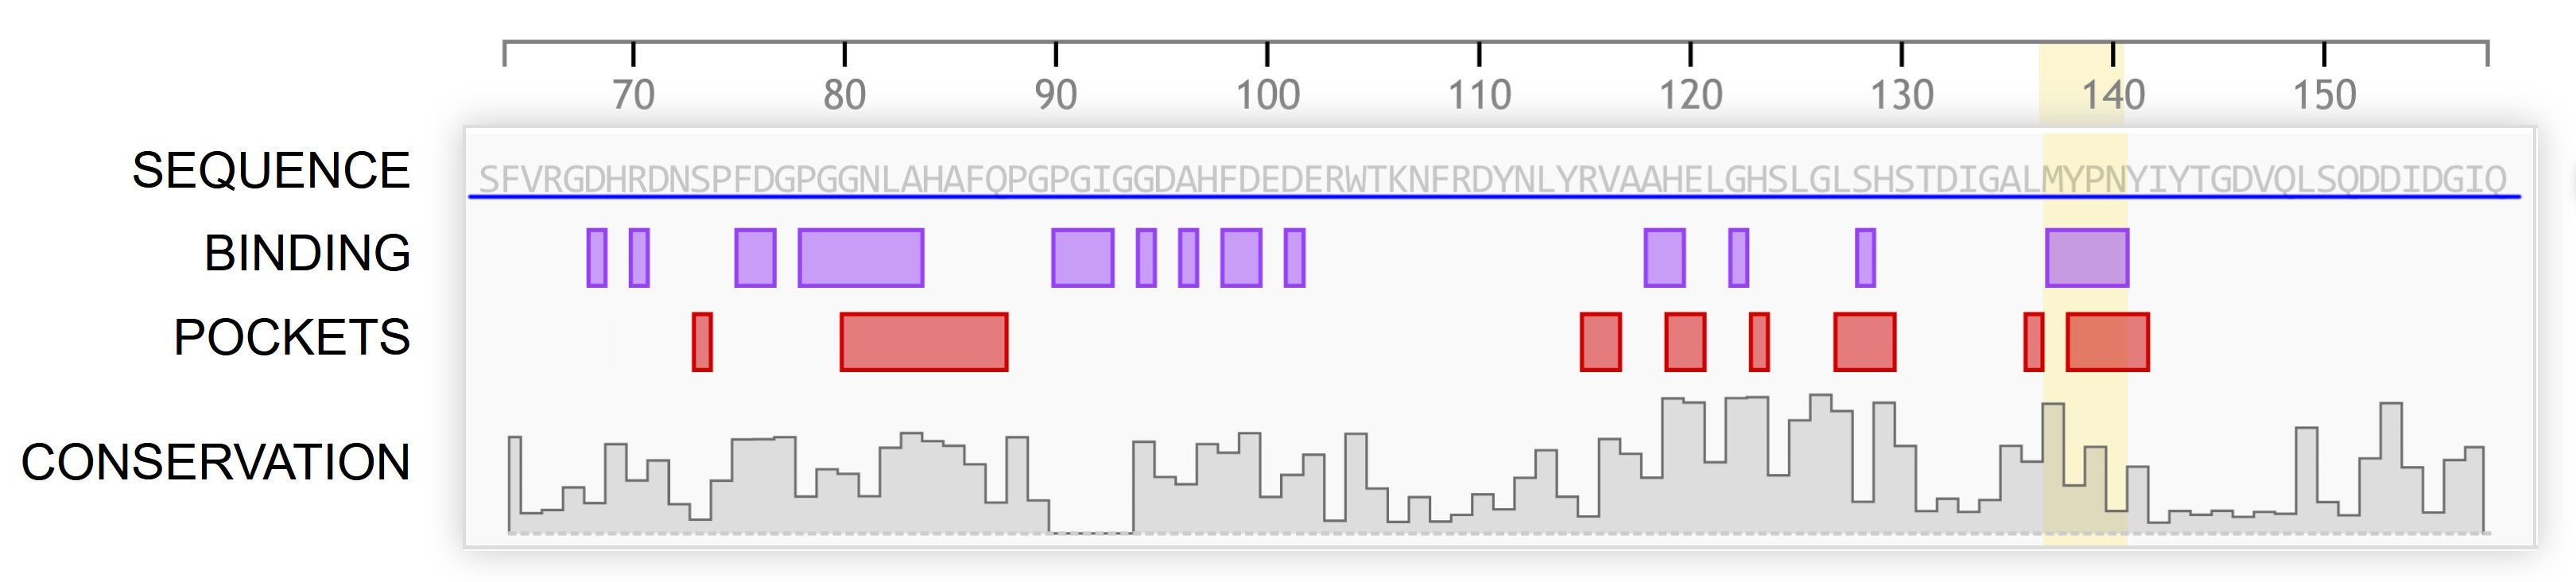
\includegraphics[width=1\linewidth]{primary_done.jpg}
    \caption{Visualization of the primary structure of the 1FBL protein. The sequence of amino acids is underlined in blue. Possible pockets and binding sites predicted by P2Rank are aligned to the sequence and shown in purple and red. Visualization was generated by \href{https://prankweb.cz/viewer?id=1fbl&database=v3-conservation-hmm}{Prank web} (\cite{prankweb}).}
    \label{fig:primary}
\end{figure}

The secondary structure is formed by the folding of the protein. Two primary substructures usually appear as alpha-helix and beta-pleated sheets, visualized in figure ~\ref{fig:secondary} The alpha-helix is a spiral beside the beta-sheet, which refers to folding pieces of the main sequence together. These constitutions are made due to hydrogen bonding between amino and carboxyl groups of peptide bonds in sequence. 

\begin{figure}%
\begin{subfigure}{0.45\textwidth}
    \centering
    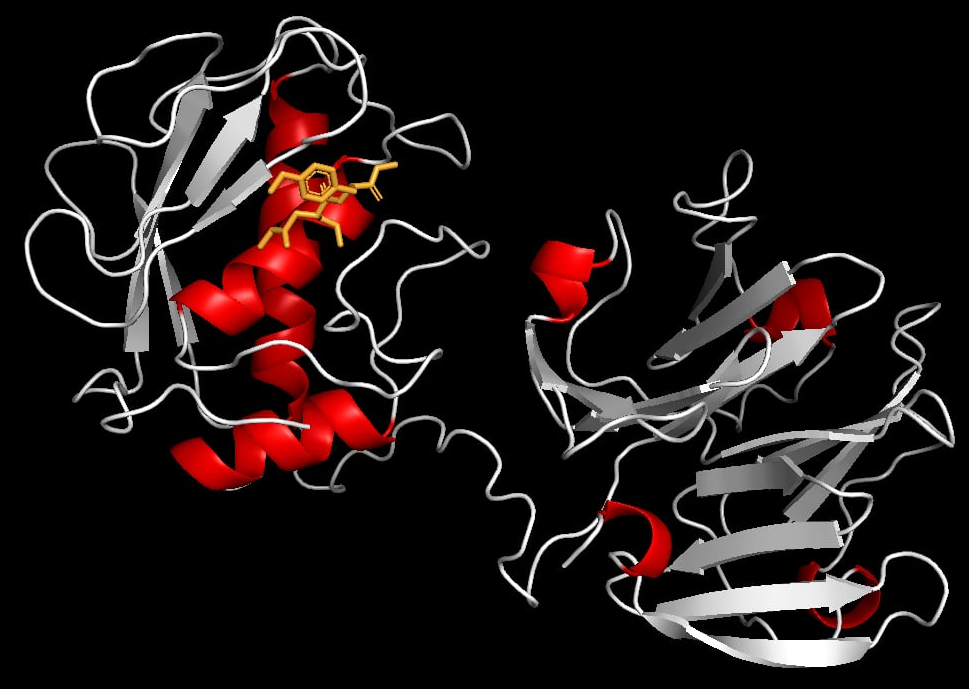
\includegraphics[width=1\linewidth]{alpha_helix.png}
    \caption{Alpha helices}
\end{subfigure}%
\begin{subfigure}{0.45\textwidth}
    \centering
    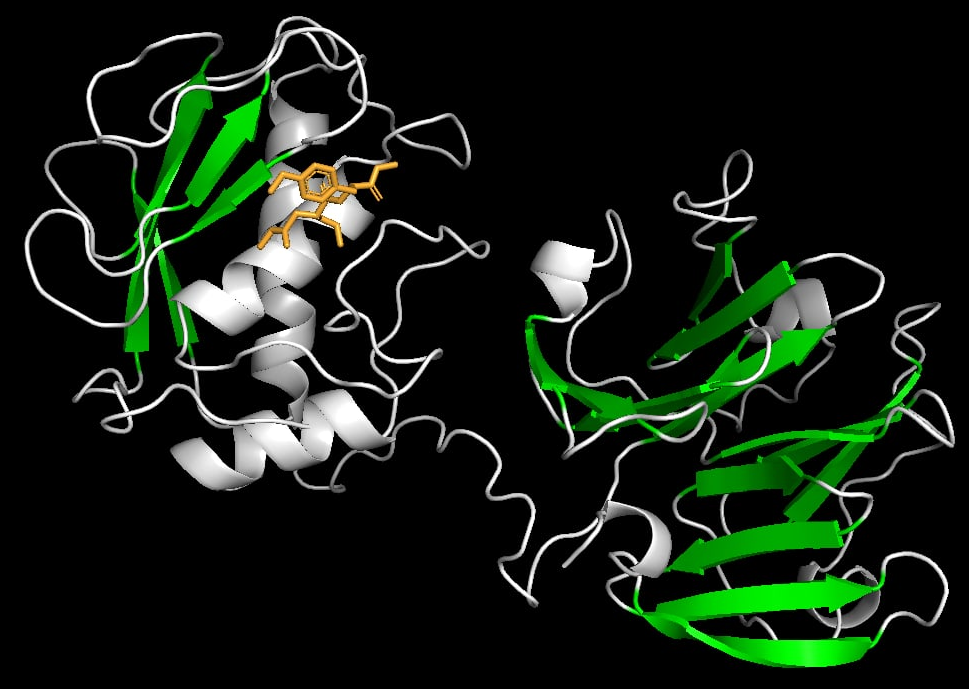
\includegraphics[width=1\linewidth]{beta_sheets.png}
    \caption{Beta sheets}
\end{subfigure}
\caption{Visualization of the secondary structure of the 1FBL protein with an attached ligand. }
\label{fig:secondary}
\end{figure}

The tertiary structure describes the overall three-dimensional arrangement of the molecule. It is determined by the lower substructures and non-covalent interactions, such as intramolecular hydrogen bonding, hydrophilic and hydrophobic interactions, and other non-covalent forces inside the molecule. This structure is essential for binding other molecules called ligands to the protein. It determines whether the surface can form a bond or whether no bond can be created. Data used in this work is described in this structure. This structure can be seen in figure ~\ref{fig:tertiary}.

\begin{figure}
    \centering
    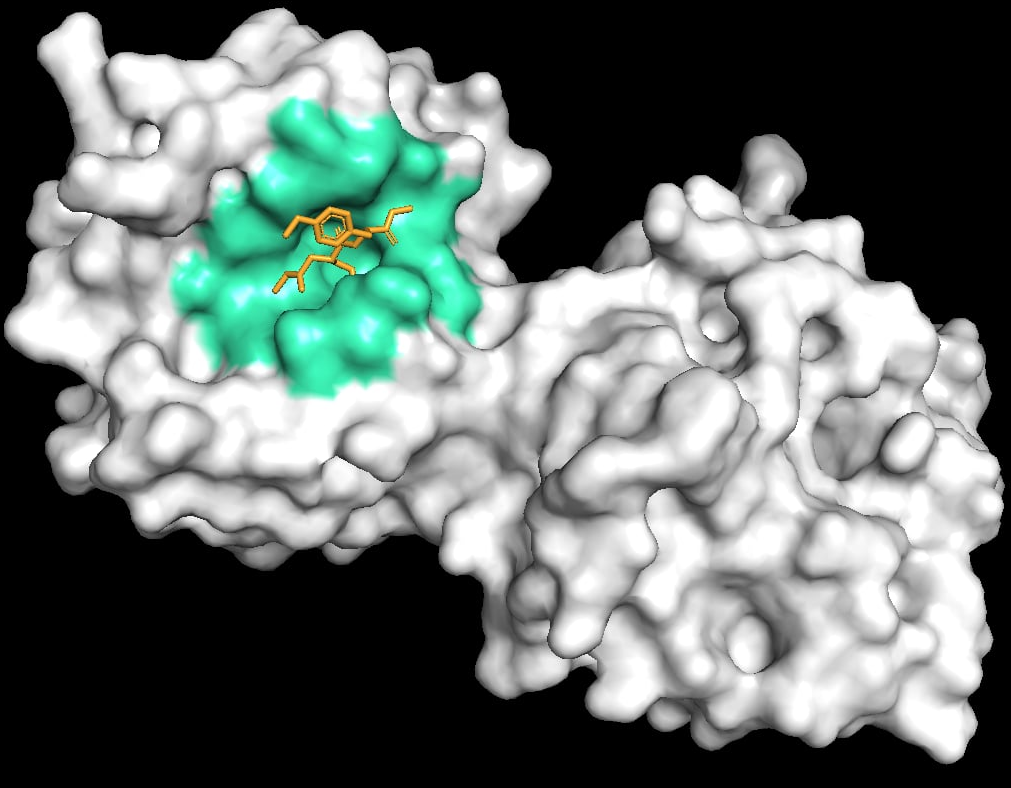
\includegraphics[width=0.5\linewidth]{tertiary.png}
    \caption{Visualization of the tertiary structure of the 1FBL protein with an \ac{LBS} highlighted in cyan with an attached ligand.}
    \label{fig:tertiary}
\end{figure}

Often, the quaternary structure is mentioned in terms of spatial organization. It is the organization of several protein subunits forming an active complex together. For instance, these subunits can be found in hemoglobin, where four molecules with hem create one greater protein complex. This structure is very similar to the tertiary one and irrelevant to the rest of this work.

More detail on this topic can be found in corresponding literature, for example, \cite{kodicek}, from which relevant parts were consulted.

\subsection{SAS points}

P2Rank (\cite{P2RANK}) works with so called \textit{solvent accessible surface} (\ac{SAS}) points. These are points on the surface of the protein (in the tertiary structure point of view), drawn by the estimated radius beyond the water molecule's van der Waals radius, checked afterward, whether they are accessible from the surface or buried in the protein. For these points, different properties can be calculated. These SAS points then form a point cloud used in this work with the described properties acting as per-point features.

\subsection{Ligand Binding Sites}
\label{LBS}

LBSs are parts of the protein where a bond with some ligand can be created. Ligand can be another protein, for instance, a receptor or enzyme. However, the precise definition differs per dataset. The applications for LBS-predictors are best described by \cite{P2RANK}:

\say{%
    Prediction LBS [...] from protein structure has many applications in [the] elucidation of protein function \cite{U1}] and rational drug design [\cite{U2},\cite{U3},\cite{U4}]. It has been employed in drug side-effects prediction [\cite{U5}], fragment-based drug discovery [\cite{U6}], docking prioritization [\cite{U7}, \cite{U8}], structure-based virtual screening [\cite{U9}], and structure-based target prediction (or so-called inverse virtual screening) [\cite{U10}]. Increasingly, LBS prediction is being used in large-scale structural studies that try to analyze and compare all known and putative binding sites on a genome-wide level [\cite{U11},\cite{U12},\cite{U13},\cite{U14},\cite{U15}]. In practice, it is often the case that predicting ligand binding sites is not an end in itself, but it represents only a step in [a] larger automated solution or pipeline.%
    }

In this work, because of limitations caused by the usage of \ac{SAS} points, only LBS on the surface can be detected, although LBS can also be on the inside part of the protein, such as ion binding sites. All the datasets used are constructed with this limitation in mind, and I will not be discussing the non-accessible LBS in this work.